\documentclass[conference]{IEEEtran}
\IEEEoverridecommandlockouts

\usepackage[T1]{fontenc}
\usepackage[utf8]{inputenc}
\usepackage{cite}
\usepackage{amsmath,amssymb}
\usepackage{graphicx}
\usepackage{booktabs}
\usepackage{array}
\usepackage{multirow}
\usepackage{xcolor}
\usepackage{tikz}
\usetikzlibrary{arrows.meta,positioning,fit,backgrounds}
\usepackage{pgfplots}
\pgfplotsset{compat=1.18}
\usepackage[hidelinks]{hyperref}
\usepackage{url}

% Results that only the planned experiments can provide are typeset in red with \tbd{}.
% See EXPERIMENT_PLAN.md for the runs that produce each number.
\newcommand{\tbd}[1]{\textcolor{red}{#1}}
\newcommand{\Mimir}{\textsc{Mimir}}

\begin{document}

\title{Do Teachers Need a Data Centre? Verifiable Exam\\Question Generation with Small Language Models\\on Consumer GPUs}

\author{
\IEEEauthorblockN{[Author 1], [Author 2], [Author 3]}
\IEEEauthorblockA{[Affiliation to be completed]\\
{[City]}, Hungary\\
{[email addresses]}}
}

\maketitle

\begin{abstract}
Large language models (LLMs) can draft exam questions from a teacher's own material, but current
tools rely on large models hosted in data centres. For schools this means recurring cost, sending
teaching material to third parties, and dependence on services they do not control. We ask whether a
single consumer graphics card with 8--12\,GB of memory is enough. Our hypothesis is that a small,
4-bit quantised model can compensate for its size with more inference-time computation: a
\emph{blueprint} pipeline plans the exam, writes one question at a time from retrieved passages with
citations, and verifies each question for grounding, distractor validity and blind answerability
before a teacher sees it. We evaluate this on 39 Hungarian and English documents with 326
human-written reference questions, against a large model on a university GPU server, measuring
question quality with a cross-family LLM judge validated by teachers, and cost as peak GPU memory,
time and energy per exam. We test whether the local pipeline is non-inferior to the server model
within a margin of half a question per ten-question exam, and whether a verified 7B model
outperforms an unverified 14B model at equal memory budget. \tbd{[Main results: quality ratio,
non-inferiority outcome, energy and time per exam.]}
\end{abstract}

\begin{IEEEkeywords}
question generation, small language models, quantisation, consumer hardware, test-time compute,
LLM-as-a-judge, educational technology, Hungarian
\end{IEEEkeywords}

\section{Introduction}

Writing multiple-choice questions is time-consuming for teachers: each question needs an unambiguous
stem, exactly one key that the course material supports, and distractors that are plausible but wrong.
LLMs can draft such questions~\cite{kurdi2020systematic,alhazmi2024distractor}, and most reported
systems rely on large models hosted in data centres. For a school this is a real constraint:
per-request cost, the transfer of teaching material (which may contain personal data) to external
processors, and availability decided elsewhere. A consumer graphics card with 8--12\,GB of memory,
by contrast, costs a few hundred euros, fits in an ordinary workstation, and keeps all data on site.

The question is whether such a card produces questions a teacher would use. It can only run models
of roughly 3--14 billion parameters, quantised to 4 or 8 bits, with a limited context. Evaluations of
quantised models report small losses on general benchmarks~\cite{li2024evalquant,kurtic2025bf16,kurt2026quant},
and small models can generate educational questions after task-specific
fine-tuning~\cite{fawzi2023small,fawzi2024towards} or with careful prompting~\cite{jaldi2026small}.
It is not known whether a quantised small model, used \emph{without} fine-tuning, can match a large
model on the full task of writing grounded exam questions from a teacher's document---especially in
a lower-resourced language such as Hungarian~\cite{ligetinagy2024hulu}---or what it costs in time
and energy on the teacher's own hardware.

We approach this as a trade between parameters and inference-time computation. Work on test-time
compute shows that a smaller model given more inference calls can outperform a larger
one~\cite{snell2025scaling}, and self-verification reduces factual errors~\cite{madaan2023selfrefine,dhuliawala2024cove}.
Exam writing suits this well: the exam structure can be planned explicitly, and each question can be
checked against its source. We therefore pair a small local model with a \emph{blueprint} pipeline
that plans, retrieves per question, cites sources and verifies, and we measure what this buys and
costs. We study four research questions:

\begin{itemize}
\item[\textbf{RQ1}] How large is the quality gap between a quantised small model on a consumer GPU
and a large server-hosted model when both use naive retrieval-augmented generation?
\item[\textbf{RQ2}] Does spending inference-time compute on planning and verification close this
gap, and at what cost in time, memory and energy per exam?
\item[\textbf{RQ3}] At a fixed memory budget, is it better to use a larger model or to spend the
same hardware on verification (7B with verification vs.\ 14B without)?
\item[\textbf{RQ4}] Does the LLM judge agree with teachers well enough to support these conclusions?
\end{itemize}

We state our expectations before running the main experiments. \textbf{H1:} with naive generation,
the server model outperforms every local model, mainly in grounding and distractor validity.
\textbf{H2:} the 4-bit 7B model with blueprint and verification is non-inferior to the server model
with naive generation. \textbf{H3:} at the 12\,GB tier, the verified 7B model outperforms the
unverified 14B model. \textbf{H4:} verification helps small models more than large ones, i.e.\ the gain
from verification shrinks as model size grows.

Our contributions are: (i) a memory-budget analysis of which model configurations fit 8 and 12\,GB
consumer GPUs for this task; (ii) a blueprint-and-verify generation pipeline designed for small
local models; (iii) a bilingual evaluation that reports quality together with peak memory, time and
energy per exam, with pre-specified non-inferiority tests against a server model; and (iv) the
open-source system, configurations and dataset manifests to reproduce it.

\section{Related Work}

\textbf{LLM-based question generation.} Surveys of educational question
generation~\cite{kurdi2020systematic} and distractor generation~\cite{alhazmi2024distractor} note that
evaluation often relies on reference-overlap metrics or small human studies that rarely verify answer
correctness. Most recent LLM studies use large proprietary models. Fawzi et al.\ showed that small
models can reach comparable quality after further pre-training and
fine-tuning~\cite{fawzi2023small,fawzi2024towards}; Jaldi et al.\ compared small and large models for
Bloom-aligned assessment design and the reliability of model-based judging~\cite{jaldi2026small}. We
differ in using off-the-shelf quantised models without fine-tuning, generating from arbitrary teacher
documents, and measuring hardware cost alongside quality.

\textbf{Quantisation and consumer hardware.} Post-training quantisation reduces memory with limited
accuracy loss: 4-bit weight-only formats are often close to 8-bit~\cite{li2024evalquant,kurtic2025bf16},
and the llama.cpp K-quants used by consumer runtimes have been evaluated systematically on 8B
models~\cite{kurt2026quant}. Energy measurements of 1--7B models on a consumer GPU show that
architecture and quantisation, not only size, determine energy per token~\cite{zahl2026energy}. These
studies use general benchmarks; we measure the cost of a complete, multi-call generation task.

\textbf{Test-time compute and verification.} Allocating more inference computation can be more
effective than scaling parameters~\cite{snell2025scaling}; iterative self-feedback~\cite{madaan2023selfrefine}
and verification questions~\cite{dhuliawala2024cove} improve factuality. Retrieval-augmented
generation~\cite{lewis2020rag} grounds outputs in documents. Our verifier combines these ideas for
exam questions: it checks each question against the passages it cites and asks the model to answer
the question blind.

\textbf{Lower-resourced languages.} Hungarian is morphologically rich and has far less training data
than English. Benchmarks such as HuLU~\cite{ligetinagy2024hulu} and question-answering corpora such as
MILQA~\cite{novak2023milqa} exist, but we know of no evaluation of exam question generation in
Hungarian, and small multilingual models are the most likely to degrade in such a language. We
therefore evaluate every system on Hungarian and English documents and report the languages
separately.

\textbf{Evaluation with LLM judges.} LLM judges scale evaluation and correlate with
humans~\cite{zheng2023judge} but prefer their own model family~\cite{panickssery2024selfpref}. We
therefore use a judge from a different family than every generator and validate it against teachers.

\section{Method}

\subsection{The memory budget of a consumer GPU}

A single consumer GPU must hold the quantised weights $W_q$, the key--value (KV) cache for the
context, and runtime buffers $R$:
\begin{equation}
M \approx W_q + 2\,L\,h_{kv}\,d_h\,b\,C + R \;\le\; M_{\mathrm{GPU}},
\end{equation}
with $L$ layers, $h_{kv}$ key--value heads of dimension $d_h$, $b$ bytes per cache element and
context length $C$. Grouped-query attention keeps the cache small for the Qwen2.5
family~\cite{qwen25}: 56\,KiB per token for the 7B model versus 128\,KiB for Llama-3.1-8B~\cite{grattafiori2024llama3}.
Table~\ref{tab:budget} applies this to the configurations we study, with $C=8{,}192$ tokens (enough
for every prompt in our pipelines) and $R\approx0.6$\,GB. A 4-bit 7B model fits an 8\,GB card with
room for the operating system; a 4-bit 14B model or an 8-bit 7B model needs a 12\,GB card. We run
text embeddings and all other services on the CPU so that the GPU holds only the language model, and
we record the measured peak memory for every exam.

\begin{table}[t]
\centering
\caption{Estimated GPU memory at an 8{,}192-token context (fp16 KV cache, $R\approx0.6$\,GB).
Measured peaks are reported with the results.}
\label{tab:budget}
\footnotesize
\setlength{\tabcolsep}{3pt}
\begin{tabular}{@{}lcccccc@{}}
\toprule
Model & Quant. & Weights & KV/token & KV@8k & Total & Tier \\
\midrule
Qwen2.5-3B  & Q4\_K\_M & 1.9\,GB & 36\,KiB  & 0.3\,GB & 2.8\,GB  & 8\,GB \\
Qwen2.5-7B  & Q4\_K\_M & 4.7\,GB & 56\,KiB  & 0.5\,GB & 5.8\,GB  & 8\,GB \\
Llama-3.1-8B & Q4\_K\_M & 4.9\,GB & 128\,KiB & 1.1\,GB & 6.6\,GB  & 8\,GB \\
Qwen2.5-7B  & Q8\_0    & 8.1\,GB & 56\,KiB  & 0.5\,GB & 9.2\,GB  & 12\,GB \\
Qwen2.5-14B & Q4\_K\_M & 9.0\,GB & 192\,KiB & 1.6\,GB & 11.2\,GB & 12\,GB \\
\bottomrule
\end{tabular}
\end{table}

\subsection{Baseline: naive retrieval-augmented generation}

The document is split into semantic chunks (sentence embeddings with multilingual
E5~\cite{wang2024me5}, cut where neighbouring sentences diverge). The three chunks most similar to the
teacher's request are retrieved, and the model writes the whole exam in one call. This is the typical
design of current tools and serves both as the baseline and, on the server, as the reference
system.

\subsection{Blueprint generation with verification}

The blueprint pipeline (Fig.~\ref{fig:pipelines}) moves work from the model's parameters to explicit
steps, each short enough for a small model and a small context.

\emph{Planning.} One call proposes $n+3$ concepts that cover the document, each with the chunks that
support it. Slots are filled greedily so that uncovered chunks are preferred, and each slot receives a
question type and a Bloom level~\cite{anderson2001bloom} drawn from a difficulty-dependent mix. The
requested number and type of questions is thus guaranteed by construction.

\emph{Per-question generation.} For each slot, the concept's chunks are combined with the top-$k$
retrieved passages, and the model writes one question that must cite the chunks supporting its key.

\emph{Verification.} Rule checks run first (answer shape, references to ``the text'', valid
citations). An LLM call then checks that the cited chunks support the key and refute every
distractor, and a second call answers the question \emph{blind}---from the cited text, without the
key---and must pick the keyed option. A failing question is regenerated once with the verifier's
feedback, then replaced by a spare concept; as a last resort the best attempt is kept and flagged for
the teacher. Near-duplicate questions are regenerated.

For a ten-question exam, the naive baseline makes one call, planning alone makes 11, and full
verification makes at least 31 (61 when every question needs its retry). The question is whether
these extra, short calls on a small model are worth more than a larger model.

\begin{figure*}[t]
\centering
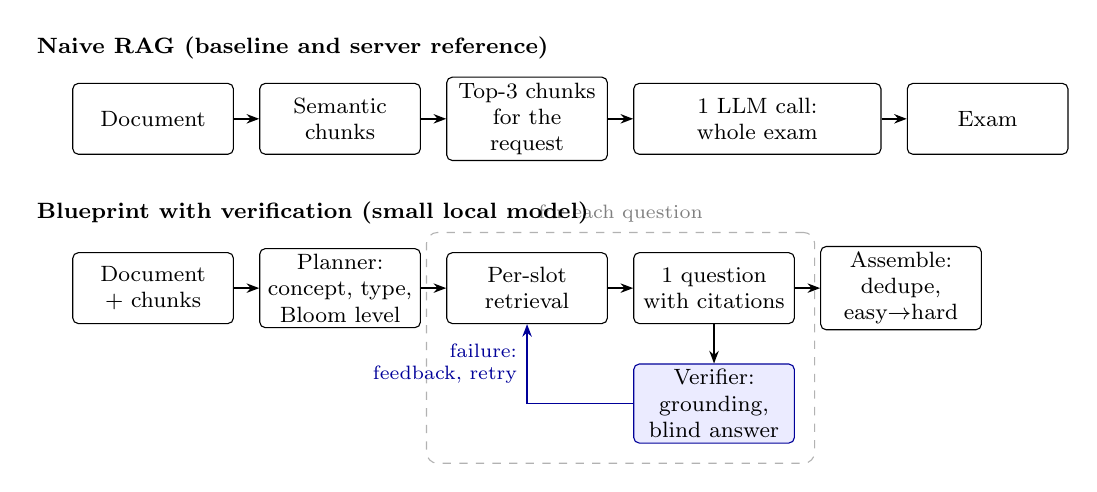
\begin{tikzpicture}[
  node distance=2.5mm and 3.2mm,
  box/.style={draw, rounded corners=2pt, align=center, font=\footnotesize, minimum height=9mm, inner sep=2pt, text width=19mm},
  hl/.style={box, fill=blue!8, draw=blue!60!black},
  arr/.style={-{Stealth[length=1.6mm]}, semithick},
  lab/.style={font=\footnotesize\bfseries, anchor=west}]
\node[lab] at (-1.2, 1.35) {Naive RAG (baseline and server reference)};
\node[box] (n1) at (0.4,0.45) {Document};
\node[box, right=of n1] (n2) {Semantic chunks};
\node[box, right=of n2] (n3) {Top-3 chunks for the request};
\node[box, right=of n3, text width=30mm] (n4) {1 LLM call: whole exam};
\node[box, right=of n4] (n5) {Exam};
\foreach \a/\b in {n1/n2,n2/n3,n3/n4,n4/n5} \draw[arr] (\a) -- (\b);
\node[lab] at (-1.2, -0.75) {Blueprint with verification (small local model)};
\node[box] (b1) at (0.4,-1.7) {Document + chunks};
\node[box, right=of b1] (b3) {Planner: concept, type, Bloom level};
\node[box, right=of b3] (b4) {Per-slot retrieval};
\node[box, right=of b4] (b5) {1 question with citations};
\node[hl, below=5mm of b5] (b6) {Verifier: grounding, blind answer};
\node[box, right=of b5] (b7) {Assemble: dedupe, easy$\to$hard};
\foreach \a/\b in {b1/b3,b3/b4,b4/b5,b5/b7} \draw[arr] (\a) -- (\b);
\draw[arr] (b5.south) -- (b6.north);
\draw[arr, blue!60!black] (b6.west) -- (b6.west -| b4.south) -- node[left, font=\scriptsize, align=right] {failure:\\feedback, retry} (b4.south);
\begin{scope}[on background layer]
\node[draw=gray!60, dashed, rounded corners, fit=(b4)(b5)(b6), inner sep=2.5mm, label={[font=\scriptsize, text=gray]above:for each question}] {};
\end{scope}
\end{tikzpicture}
\caption{The two generation strategies. The blueprint replaces one long call by many short calls
(planning, one question at a time, verification), trading inference computation for model size.}
\label{fig:pipelines}
\end{figure*}

\subsection{Deployment configuration}

All local models run in the Ollama runtime with GGUF weights. Q4\_K\_M is a 4-bit ``K-quant'' that
keeps selected tensors at higher precision and is the default for consumer use; Q8\_0 is an 8-bit
format close to the unquantised model~\cite{kurt2026quant}. Only one model is resident on the GPU at a
time and requests are processed one by one, so the generator never competes with another model for
memory; the verifier uses the same model as the generator with a different prompt, which avoids
swapping models between steps. The E5 embedding model, the vector index and all services run on the
CPU. The context is set per request to 8{,}192 tokens; the longest prompt in either pipeline, a planning
call over a 12{,}000-character overview of the document, stays within it.

\section{Experimental Setup}

\subsection{Data}

Table~\ref{tab:dataset} summarises the 39 documents. English documents come from OpenStax textbooks
via EduQG~\cite{hadifar2023eduqg} and Hungarian ones from Wikipedia via MILQA~\cite{novak2023milqa},
selected as short, medium and long and filtered to reference questions whose evidence sentence occurs
in the document; three short Hungarian teaching texts were written by the authors. Reference questions
are used for retrieval recall and similarity, not as generation targets. The dataset is frozen before
the main runs.

\begin{table}[t]
\centering
\caption{Evaluation data: 39 documents, 326 reference questions.}
\label{tab:dataset}
\footnotesize
\setlength{\tabcolsep}{3.5pt}
\begin{tabular}{@{}llrcrr@{}}
\toprule
Source & Lang & Docs & S/M/L & Median chars & Ref.\ Q \\
\midrule
Own teaching texts & HU & 3 & 3/0/0 & 1{,}923 & 12 \\
OpenStax via EduQG & EN & 12 & 4/4/4 & 16{,}752 & 74 \\
Wikipedia via MILQA & HU & 24 & 8/8/8 & 8{,}072 & 240 \\
\midrule
Total & & 39 & 15/12/12 & 7{,}919 & 326 \\
\bottomrule
\end{tabular}
\end{table}

\subsection{Systems and hardware}

Table~\ref{tab:systems} lists the compared systems. Local systems run in Ollama with GGUF weights on
an 8\,GB (\tbd{RTX 3070 Ti}) or 12\,GB (\tbd{RTX 3060}) card, one request at a time, temperature 0.2,
an 8{,}192-token context. The server reference runs a large \tbd{[model, size]} on the university's
GPU server. Each system writes a ten-question multiple-choice exam per document, with three seeds for
single-call systems and one for the multi-call ones.

\begin{table}[t]
\centering
\caption{Hardware and measurement protocol.}
\label{tab:hw}
\footnotesize
\setlength{\tabcolsep}{3pt}
\begin{tabular}{@{}>{\raggedright\arraybackslash}p{2.0cm}>{\raggedright\arraybackslash}p{6.0cm}@{}}
\toprule
Item & Setting \\
\midrule
8\,GB tier & \tbd{GPU, CPU, RAM, driver, OS} \\
12\,GB tier & \tbd{GPU, CPU, RAM, driver, OS} \\
Runtime & Ollama \tbd{version}, GGUF, context 8{,}192, one request at a time \\
Warm-up & One unmeasured exam per system to load the model \\
Memory & Peak used GPU memory, sampled every 0.5\,s; idle baseline recorded \\
Energy & Board power at 2\,Hz, integrated per exam; idle power subtracted and reported \\
Offloading & Runtime report checked: 100\,\% of layers on the GPU, else the run is marked \\
\bottomrule
\end{tabular}
\end{table}

\begin{table}[t]
\centering
\caption{Compared systems. L = local consumer GPU, S = university GPU server.}
\label{tab:systems}
\footnotesize
\setlength{\tabcolsep}{2.5pt}
\begin{tabular}{@{}llll@{}}
\toprule
ID & Model (quantisation) & Pipeline & GPU \\
\midrule
L7-naive & Qwen2.5-7B (Q4\_K\_M) & naive RAG & 8\,GB \\
L7-plan & Qwen2.5-7B (Q4\_K\_M) & blueprint, no verifier & 8\,GB \\
L7-verify & Qwen2.5-7B (Q4\_K\_M) & blueprint + verifier & 8\,GB \\
L3-verify & Qwen2.5-3B (Q4\_K\_M) & blueprint + verifier & 8\,GB \\
L8-verify & Llama-3.1-8B (Q4\_K\_M) & blueprint + verifier & 8\,GB \\
L7q8-verify & Qwen2.5-7B (Q8\_0) & blueprint + verifier & 12\,GB \\
L14-naive & Qwen2.5-14B (Q4\_K\_M) & naive RAG & 12\,GB \\
L14-verify & Qwen2.5-14B (Q4\_K\_M) & blueprint + verifier & 12\,GB \\
S-naive & \tbd{server model} & naive RAG & server \\
S-verify & \tbd{server model} & blueprint + verifier & server \\
\bottomrule
\end{tabular}
\end{table}

\subsection{Measures}

\textbf{Quality.} Per exam, \emph{format compliance} is 1 if the exam has exactly the requested
number and shape of questions (unparsable output and error placeholders count as failures). Per
question, the judge decides \emph{grounding} (the source supports the key; it must quote the
supporting sentence), \emph{distractor validity} (each distractor is false and on topic), and
\emph{blind answerability} (answering from the source without the key picks the keyed option), and
gives 1--5 scores for correctness, clarity, distractor quality and Bloom fit. The \emph{quality index}
is the mean of the four binary-based rates. Automatic measures add duplicate rate, section coverage
and retrieval recall against the reference evidence.

\textbf{Cost.} For every exam we record wall-clock time, LLM calls and tokens, output throughput
(tokens/s from the runtime), peak GPU memory, and GPU energy, integrated from board power sampled at
2\,Hz with \texttt{nvidia-smi} as in~\cite{zahl2026energy}; idle power is measured before each run and
reported separately.

\textbf{Judge and teachers.} The judge is gpt-oss-120b~\cite{gptoss2025}, a different model family
from all generators, run on the server only for evaluation. Three teachers rate a blind, shuffled
sample of 15 questions per system on the same rubric; Krippendorff's $\alpha$~\cite{krippendorff2004}
measures their agreement, and Spearman's $\rho$ and Cohen's $\kappa$ measure agreement between judge
and teachers.

\subsection{Analysis}

Documents are the unit of analysis: measures are averaged over questions and seeds per document. We
report means with 95\,\% bootstrap confidence intervals over documents~\cite{efron1993}.

\emph{Differences} (RQ1, RQ3) are tested with paired Wilcoxon signed-rank tests~\cite{wilcoxon1945},
Holm-corrected~\cite{holm1979}, with the rank-biserial correlation as effect size~\cite{kerby2014}.

\emph{Non-inferiority} (RQ2): the local system is non-inferior to the server reference if the lower
bound of the one-sided 95\,\% bootstrap interval of the paired difference in quality index lies above
$-\delta$, with $\delta=0.05$ fixed in advance. Since each component is a rate over ten questions,
$\delta$ corresponds to half a question per exam. We also report the \emph{gap closure}
$(Q_{\text{L-verify}}-Q_{\text{L-naive}})/(Q_{\text{S-naive}}-Q_{\text{L-naive}})$.

\emph{Measurement validity.} Two defects found while building the harness would have biased the
comparison and are fixed: a hard-coded error exam returned when all model calls failed was counted as
a result, and the chunker embedded only the first 512 tokens of each document---an estimated
68--71\,\% of the average dataset document received no semantic signal. The error exam is now flagged
and counted as a failure, and the chunker works in 512-token windows.

\section{Results}
\label{sec:results}

\tbd{All numbers in this section are produced by the experiments in EXPERIMENT\_PLAN.md; red values
are placeholders.}

\begin{table}[t]
\centering
\caption{Quality and cost per system (document means). Index with 95\,\% CI.}
\label{tab:main}
\footnotesize
\setlength{\tabcolsep}{2.2pt}
\begin{tabular}{@{}lcccccc@{}}
\toprule
System & Index [CI] & Ground. & Blind & VRAM & min/exam & Wh/exam \\
\midrule
L7-naive    & \tbd{--} & \tbd{--} & \tbd{--} & \tbd{--} & \tbd{--} & \tbd{--} \\
L7-plan     & \tbd{--} & \tbd{--} & \tbd{--} & \tbd{--} & \tbd{--} & \tbd{--} \\
L7-verify   & \tbd{--} & \tbd{--} & \tbd{--} & \tbd{--} & \tbd{--} & \tbd{--} \\
L3-verify   & \tbd{--} & \tbd{--} & \tbd{--} & \tbd{--} & \tbd{--} & \tbd{--} \\
L8-verify   & \tbd{--} & \tbd{--} & \tbd{--} & \tbd{--} & \tbd{--} & \tbd{--} \\
L7q8-verify & \tbd{--} & \tbd{--} & \tbd{--} & \tbd{--} & \tbd{--} & \tbd{--} \\
L14-naive   & \tbd{--} & \tbd{--} & \tbd{--} & \tbd{--} & \tbd{--} & \tbd{--} \\
L14-verify  & \tbd{--} & \tbd{--} & \tbd{--} & \tbd{--} & \tbd{--} & \tbd{--} \\
S-naive     & \tbd{--} & \tbd{--} & \tbd{--} & --       & \tbd{--} & --       \\
S-verify    & \tbd{--} & \tbd{--} & \tbd{--} & --       & \tbd{--} & --       \\
\bottomrule
\end{tabular}
\end{table}

\begin{figure}[t]
\centering
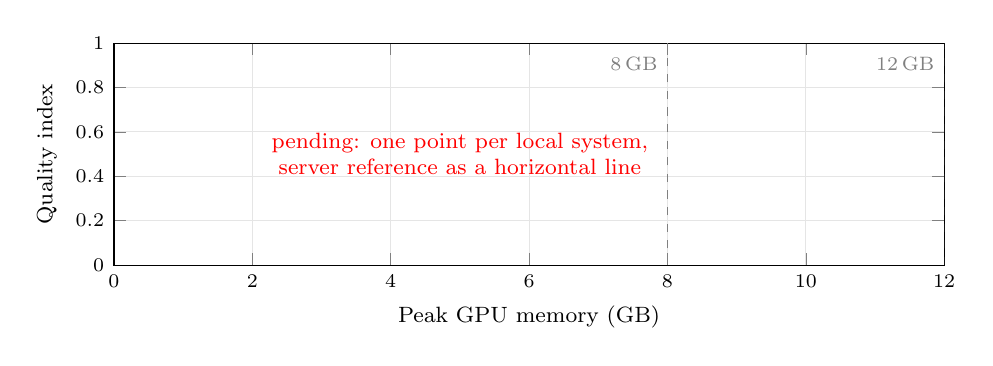
\begin{tikzpicture}
\begin{axis}[
  width=\columnwidth, height=4.4cm,
  xmin=0, xmax=12, ymin=0, ymax=1,
  xlabel={Peak GPU memory (GB)}, ylabel={Quality index},
  xlabel style={font=\footnotesize}, ylabel style={font=\footnotesize},
  tick label style={font=\scriptsize}, grid=major, grid style={gray!20}]
\addplot[dashed, gray] coordinates {(8,0) (8,1)};
\addplot[dashed, gray] coordinates {(12,0) (12,1)};
\node[font=\scriptsize, text=gray, anchor=north east] at (axis cs:8,0.98) {8\,GB};
\node[font=\scriptsize, text=gray, anchor=north east] at (axis cs:12,0.98) {12\,GB};
\node[font=\footnotesize, text=red, align=center] at (axis cs:5,0.5) {pending: one point per local system,\\server reference as a horizontal line};
\end{axis}
\end{tikzpicture}
\caption{Quality versus peak GPU memory. \tbd{Filled after the main runs.}}
\label{fig:pareto}
\end{figure}

\textbf{RQ1: the gap.} Comparing L7-naive and L14-naive with S-naive shows how much quality a
consumer GPU loses when the model is simply asked for the exam. We report the paired difference in
quality index and its components, and whether the loss lies in grounding, distractors or format.
\tbd{[Result.]}

\textbf{RQ2: closing the gap.} L7-verify is compared with S-naive under the non-inferiority criterion,
and the gap closure is reported with the time, memory and energy it costs (Table~\ref{tab:main},
Fig.~\ref{fig:pareto}). L7-plan separates the effect of planning from that of verification.
\tbd{[Result.]}

\begin{table}[t]
\centering
\caption{Where the time goes: share of calls and time per stage for L7-verify (median exam).}
\label{tab:stages}
\footnotesize
\begin{tabular}{@{}lccc@{}}
\toprule
Stage & Calls & Time share & Output tokens \\
\midrule
Planning & 1 & \tbd{--} & \tbd{--} \\
Question writing & \tbd{--} & \tbd{--} & \tbd{--} \\
Grounding check & \tbd{--} & \tbd{--} & \tbd{--} \\
Blind answer & \tbd{--} & \tbd{--} & \tbd{--} \\
Retries and replacements & \tbd{--} & \tbd{--} & \tbd{--} \\
\bottomrule
\end{tabular}
\end{table}

The cost of verification is broken down by stage in Table~\ref{tab:stages}; this shows which check
could be dropped or made adaptive if time matters more than the last points of quality, and it
converts the time per exam into a capacity estimate (exams per GPU-hour).

\textbf{RQ3: parameters or verification.} At the 12\,GB tier, L14-naive and L7-verify (or
L7q8-verify) use comparable memory. If verification is the better use of the hardware,
L7-verify should outperform L14-naive; L14-verify shows whether the two add up, and L3-verify and
L8-verify show how far down in size and across model families the effect holds.
\tbd{[Result.]}

\textbf{RQ4: judge validity.} Table~\ref{tab:agree} reports teacher agreement and judge--teacher
agreement per criterion. \tbd{[Result.]} If judge--teacher agreement is low for a criterion, conclusions
for that criterion are drawn from the teacher ratings only.

\begin{table}[t]
\centering
\caption{Agreement between teachers ($\alpha$) and between judge and teachers ($\rho$, $\kappa$).}
\label{tab:agree}
\footnotesize
\begin{tabular}{@{}lccc@{}}
\toprule
Criterion & Teachers $\alpha$ & Judge--teacher $\rho$ & $n$ \\
\midrule
Correctness & \tbd{--} & \tbd{--} & \tbd{--} \\
Clarity & \tbd{--} & \tbd{--} & \tbd{--} \\
Distractor quality & \tbd{--} & \tbd{--} & \tbd{--} \\
Bloom fit & \tbd{--} & \tbd{--} & \tbd{--} \\
Would use (yes/no) & \tbd{--} & -- & \tbd{--} \\
\midrule
\multicolumn{2}{@{}l}{Grounded vs.\ teacher correctness $\ge 4$ ($\kappa$)} & \tbd{--} & \tbd{--} \\
\bottomrule
\end{tabular}
\end{table}

\textbf{Error analysis.} For each system we inspect the questions that failed grounding or the blind
test and code the failure: key not in the source, two defensible options, distractor true, question
answerable without the source, or wrong language or format. The distribution of these codes shows
whether small models fail differently from the server model, which matters for how much a teacher's
review has to catch. \tbd{[Result.]}

\textbf{Language.} All analyses are repeated for the Hungarian and English subsets. Because the
subsets differ in source and length, differences between languages are descriptive.

\section{Discussion}

\textbf{What the answer means for schools.} If the non-inferiority test succeeds, a school can write
exams of comparable quality on a workstation GPU, at the energy and waiting time reported in
Table~\ref{tab:main}, without sending teaching material off site. If it fails, the size of the gap and
where it lies (grounding, distractors, format) show whether a teacher's review can realistically
absorb it, and whether a 12\,GB card is the minimum. A single consumer GPU processes one exam at a time;
scaling to many concurrent users requires more GPUs or a server, which is an operational rather than
a research question.

\textbf{Why structure should help small models.} Each step of the blueprint pipeline needs only a
short context and a narrow skill---proposing concepts, writing one question, judging support for one
key---while the naive prompt asks for planning, writing and self-consistency in one pass over a long
output. The same property keeps the KV cache small, which is what makes the 8\,GB tier possible.

\textbf{Threats to validity.} \emph{Internal:} the multi-call systems run one seed per document and the
single-call systems three, so their seed variance is estimated differently; the server's load and the
consumer GPU's thermal state can affect time and energy, which is why we warm up, subtract idle power
and report medians. \emph{Construct:} the judge sees only each question's cited context and may miss
contradictions elsewhere in the document, and the quality index weights its four components equally;
the teacher rating and per-component results guard against both. Energy is measured at the GPU board
and excludes the rest of the machine. \emph{External:} the evaluation covers multiple-choice questions
from 39 documents; Wikipedia and textbook text is cleaner than typical lecture notes; Hungarian and
English documents come from different sources; and the results hold for the models and runtime
version tested, which change quickly. We do not fine-tune; fine-tuned small
models~\cite{fawzi2024towards} may close the gap at lower inference cost and are complementary.

\section{Conclusion}

We asked whether exam generation needs a data centre. We formulated the memory budget of the task on
8 and 12\,GB consumer GPUs, designed a pipeline that trades model size for short, verifiable
inference steps, and set up a bilingual evaluation that measures quality together with memory, time
and energy per exam, with a pre-specified non-inferiority margin against a large server model.
\tbd{[Summary of findings.]} The code, configurations and dataset manifests are released for
reproduction.

\section*{Ethical Considerations}
Local processing keeps teaching material on the school's hardware; uploaded documents are deleted
after each job, and no student data is processed. All generated questions require teacher review
before use, and exported exams state that they were drafted with an AI system and by which model, in
line with the transparency and human-oversight duties of the EU AI Act~\cite{aiact2024}. The
evaluation documents are the authors' own or openly licensed (CC~BY~4.0, CC~BY-SA~4.0).

\section*{Acknowledgment}
[To be completed: funding, access to the university GPU server, teacher raters.]

\bibliographystyle{IEEEtran}
\bibliography{references}

\end{document}
